\documentclass[final]{beamer}

\usepackage[T1]{fontenc}
 \usepackage[utf8]{luainputenc}
\usepackage{lmodern}
\usepackage[size=custom, width=122,height=91, scale=1.2]{beamerposter}
\usetheme{gemini}
\usecolortheme{bgu}
\usepackage{graphicx}
\usepackage{booktabs}
\usepackage{tikz}
\usepackage{pgfplots}
\pgfplotsset{compat=1.14}
%\usepackage{anyfontsize}


\newlength{\sepwidth}
\newlength{\colwidth}
\setlength{\sepwidth}{0.025\paperwidth}
\setlength{\colwidth}{0.3\paperwidth}

\newcommand{\separatorcolumn}{\begin{column}{\sepwidth}\end{column}}



\title{Rubik's Mathematics: A Twist on Numbers}

\author{Jeremy Huang and Benedict Antonious}

\institute[shortinst]{University of Colorado Boulder}



\logoleft{
\includegraphics[height=4.5cm]{logos/BoulderLogo.png}}


\begin{document}

\begin{frame}[t]
\begin{columns}[t]
\separatorcolumn

\begin{column}{\colwidth}

  \begin{block}{Abstract}
    \large The Rubik's Cube, an iconic 3D puzzle, has captured the imagination of enthusiasts and mathematicians alike for decades. This poster delves into the mathematical intricacies of the Rubik's Cube. We investigate the cube's symmetry, its staggering number of possible permutations, and the use of computer aided proof-assistants to calculate the algorithms to solve the Rubik's Cube. Whether you're a puzzle enthusiast or a math fanatic, this poster invites you to embark on a fascinating journey into the world of Rubik's Cube mathematics.


  \end{block}

  \begin{block}{Combinations of a Rubik's Cube}

    \large There are three (four if you count the not-visible core) types of pieces:

    \begin{itemize} %Talk about centers/edges/corners
      \item \textbf{Corners:} 8 of these on each corner of the cube
      \item \textbf{Edges:} 12 of these connecting adjacent corners
      \item \textbf{Centers:} 6 of these on each face of the cube
    \end{itemize}

    There are $8!$ ways we can permute the corner pieces to the corners of a cube, and $12!$ ways 
    we can permute the edge pieces into the 12 edge slots of a cube. There are $3^8$ ways we can orient 
    the corner pieces and $2^{12}$ ways we can the edge pieces. We also have to divide by $12$, 
    since some states are impossible. This yields the final formula: \\

    $$ \displaystyle\frac{8!\cdot 12! \cdot 3^8 \cdot 2^{12}}{12} = 43252003274489856000 $$ \\

    \begin{figure}
      \centering
                    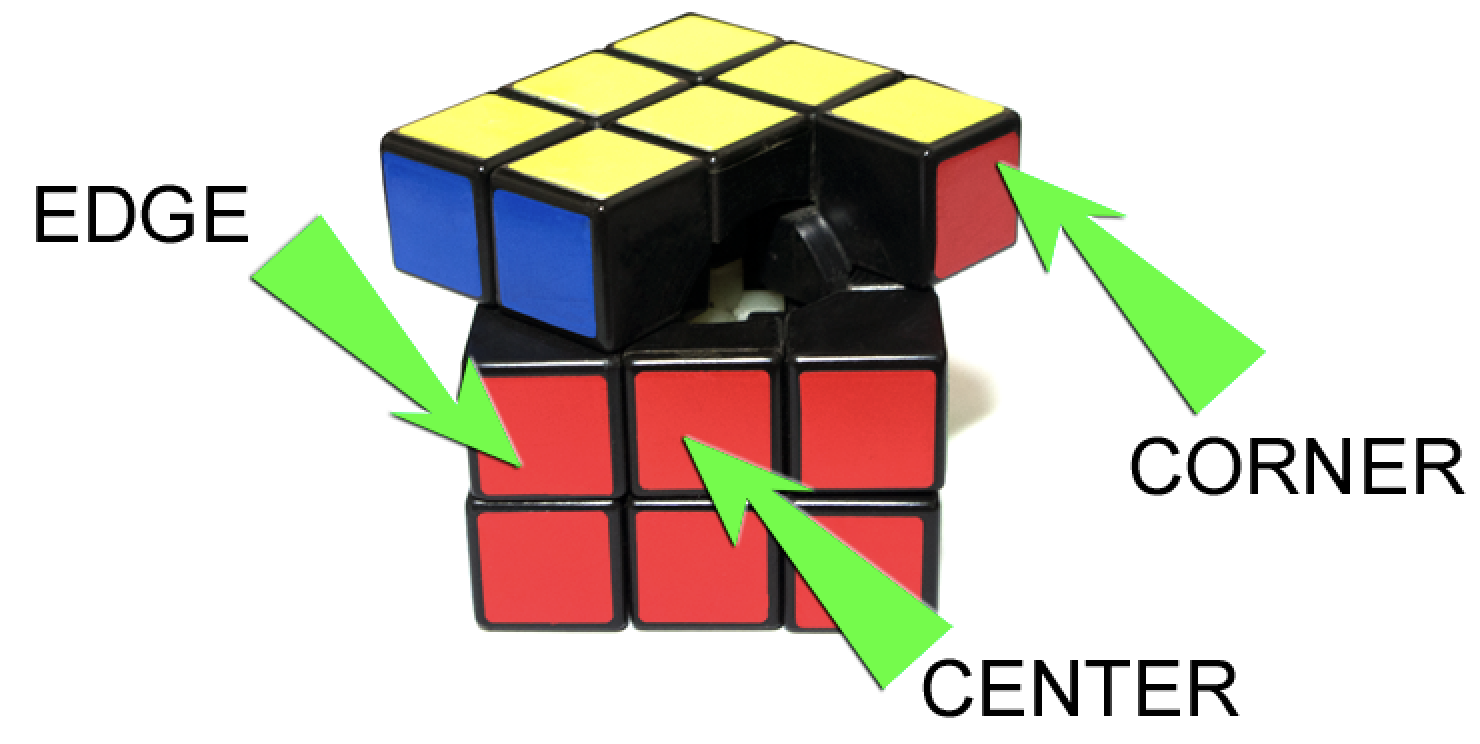
\includegraphics[width=0.6\textwidth]{logos/rubikspieces.png}
    \end{figure}

  \end{block}

  \begin{block}{How big is 43 Quintillion?}

    \large 
    %Imagine we find a new, unique Rubik's cube combination every second. There are
    %about 31 million seconds in a year, so it would take more than 1.3 trillion years. \\
    %Imagine we started doing this during the Dinosaur Age: we would only get to 2 quadrillion combinations. \\
    %We would have to repeat the process more than 20,000 times to reach all 43 quintillion combinations! \\
    Imagine we had a dollar for each rubik's cube combination there was. If were to lay one layer of one dollar bills in
    Colorado, it would take 25 trillion dollars. We would have to stack that another 2 million times to use all of our money. \\
    The stack would be about the same height of the tallest building in Denver. In other words,
    the money would cover all of Colorado in a layer as tall as a skyscraper.
    \begin{figure}
      \centering
                    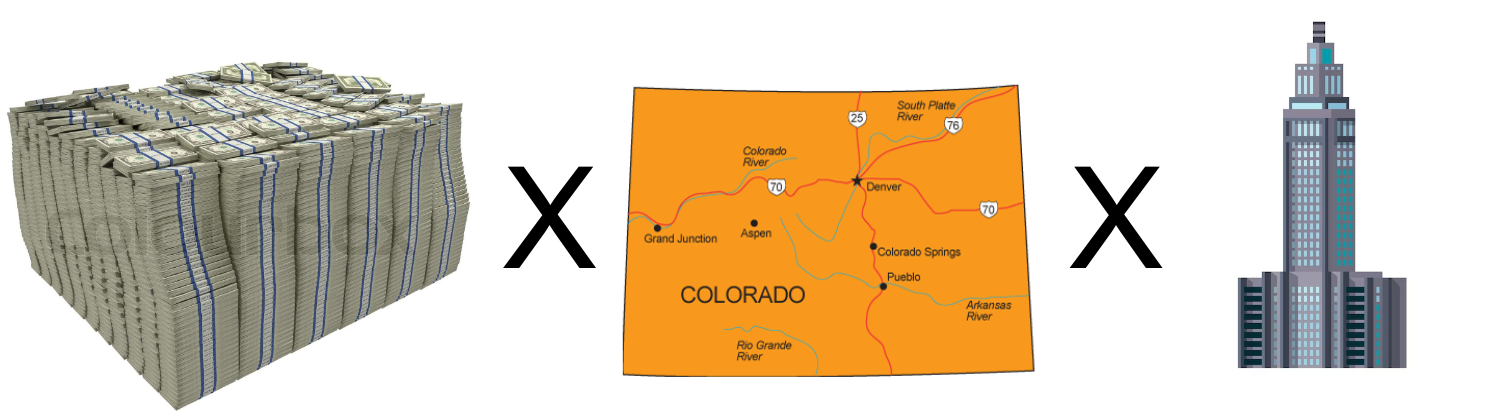
\includegraphics[width=0.9\textwidth]{logos/moneyvisual.png}
    \end{figure}

  \end{block}

\end{column}

\separatorcolumn

\begin{column}{\colwidth}

  \begin{block}{Solving a Rubik's Cube}

    \large Vivamus congue volutpat elit non semper. Praesent molestie nec erat ac
    interdum. In quis suscipit erat. \textbf{Phasellus mauris felis, molestie
    ac pharetra quis}, tempus nec ante. Donec finibus ante vel purus mollis
    fermentum. Sed felis mi, pharetra eget nibh a, feugiat eleifend dolor. Nam
    mollis condimentum purus quis sodales. Nullam eu felis eu nulla eleifend
    bibendum nec eu lorem. Vivamus felis velit, volutpat ut facilisis ac,
    commodo in metus.

    \begin{enumerate}
      \item \textbf{Morbi mauris purus}, egestas at vehicula et, convallis
        accumsan orci. Orci varius natoque penatibus et magnis dis parturient
        montes, nascetur ridiculus mus.
      \item \textbf{Cras vehicula blandit urna ut maximus}. Aliquam blandit nec
        massa ac sollicitudin. Curabitur cursus, metus nec imperdiet bibendum,
        velit lectus faucibus dolor, quis gravida metus mauris gravida turpis.
      \item \textbf{Vestibulum et massa diam}. Phasellus fermentum augue non
        nulla accumsan, non rhoncus lectus condimentum.
    \end{enumerate}

  \end{block}

  \begin{block}{God's Algorithm and Number}

    \large Et rutrum ex euismod vel. Pellentesque ultricies, velit in fermentum
    vestibulum, lectus nisi pretium nibh, sit amet aliquam lectus augue vel
    velit. Suspendisse rhoncus massa porttitor augue feugiat molestie. Sed
    molestie ut orci nec malesuada. Sed ultricies feugiat est fringilla
    posuere.

    \begin{figure}
      \centering
        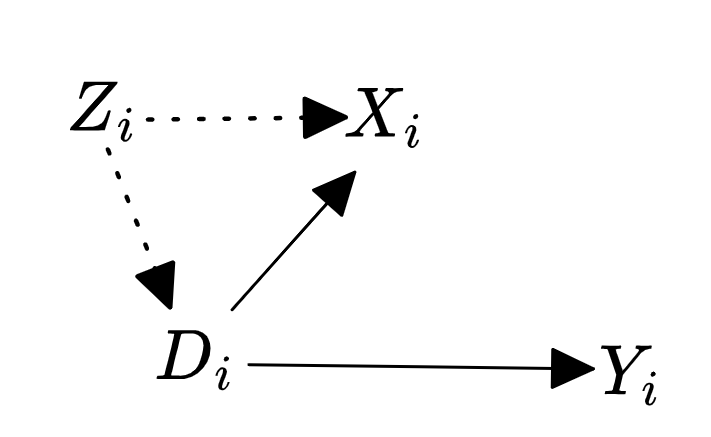
\includegraphics[width=0.3\textwidth]{figures/dag.png}

      \caption{Another figure caption.}
    \end{figure}

  \end{block}

  \begin{block}{Proof Assistants/Computer Aided proof}

    \large Nulla eget sem quam. Ut aliquam volutpat nisi vestibulum convallis. Nunc a
    lectus et eros facilisis hendrerit eu non urna. Interdum et malesuada fames
    ac ante \textit{ipsum primis} in faucibus. Etiam sit amet velit eget sem
    euismod tristique. Praesent enim erat, porta vel mattis sed, pharetra sed
    ipsum. Morbi commodo condimentum massa, \textit{tempus venenatis} massa
    hendrerit quis. Maecenas sed porta est. Praesent mollis interdum lectus,
    sit amet sollicitudin risus tincidunt non.

  \end{block}

\end{column}

\separatorcolumn

\begin{column}{\colwidth}

  \begin{exampleblock}{Statistics of Speed Cubing}

    \large

    $$
    \int_{-\infty}^{\infty} e^{-x^2}\,dx = \sqrt{\pi}
    $$

    Interdum et malesuada fames $\{1, 4, 9, \ldots\}$ ac ante ipsum primis in
    faucibus. Cras eleifend dolor eu nulla suscipit suscipit. Sed lobortis non
    felis id vulputate.

    \heading{A heading inside a block}

    Praesent consectetur mi $x^2 + y^2$ metus, nec vestibulum justo viverra
    nec. Proin eget nulla pretium, egestas magna aliquam, mollis neque. Vivamus
    dictum $\mathbf{u}^\intercal\mathbf{v}$ sagittis odio, vel porta erat
    congue sed. Maecenas ut dolor quis arcu auctor porttitor.

    \heading{Another heading inside a block}

    Sed augue erat, scelerisque a purus ultricies, placerat porttitor neque.
    Donec $P(y \mid x)$ fermentum consectetur $\nabla_x P(y \mid x)$ sapien
    sagittis egestas. Duis eget leo euismod nunc viverra imperdiet nec id
    justo.

  \end{exampleblock}

  \begin{block}{What about larger Rubik's Cubes?}

    \large Class aptent taciti sociosqu ad litora torquent per conubia nostra, per
    inceptos himenaeos. Phasellus libero enim, gravida sed erat sit amet,
    scelerisque congue diam. Fusce dapibus dui ut augue pulvinar iaculis.

    \begin{table}
      \centering
      \begin{tabular}{l r r c}
        \toprule
        \textbf{First column} & \textbf{Second column} & \textbf{Third column} & \textbf{Fourth} \\
        \midrule
        Foo & 13.37 & 384,394 & $\alpha$ \\
        Bar & 2.17 & 1,392 & $\beta$ \\
        Baz & 3.14 & 83,742 & $\delta$ \\
        Qux & 7.59 & 974 & $\gamma$ \\
        \bottomrule
      \end{tabular}
      \caption{A table caption.}
    \end{table}

    Donec quis posuere ligula. Nunc feugiat elit a mi malesuada consequat. Sed
    imperdiet augue ac nibh aliquet tristique. Aenean eu tortor vulputate,
    eleifend lorem in, dictum urna. Proin auctor ante in augue tincidunt
    tempor. Proin pellentesque vulputate odio, ac gravida nulla posuere
    efficitur. Aenean at velit vel dolor blandit molestie. Mauris laoreet
    commodo quam, non luctus nibh ullamcorper in. Class aptent taciti sociosqu
    ad litora torquent per conubia nostra, per inceptos himenaeos.



  \end{block}

  \begin{block}{References}

    \nocite{*}
    \footnotesize{\bibliographystyle{plain}\bibliography{poster}}

  \end{block}

\end{column}

\separatorcolumn
\end{columns}
\end{frame}

\end{document}
